\begin{lemma}[7.4.2]
\label{IV.2.s7.4.2-fr}
Sean $A$ y $A'$ anillos locales noetherianos, y
$\varphi:A\to A'$ un homomorfismo local tal que
$f={}^a\varphi:\operatorname{Spec}(A')\to\operatorname{Spec}(A)$
sea un $\boldsymbol P$-morfismo. Entonces, si las fibras formales
de $A'$ son geométricamente regulares, $A$ es un
$\boldsymbol P$-anillo.
\end{lemma}

\oldpage[IV-2]{199}

\begin{proof}
Consideremos el homomorfismo completado
$\widehat\varphi:\widehat A\to\widehat{A}'$ y el morfismo
correspondiente $\widehat f={}^a\widehat\varphi$; se tiene el
diagrama conmutativo
\[
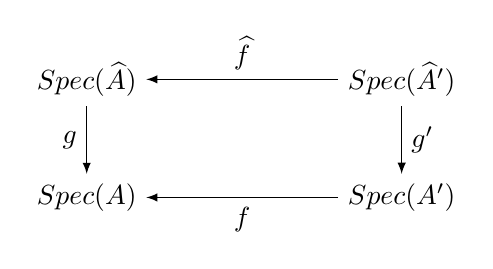
\begin{tikzpicture}[>=latex]
\node (tl) at (0,1.5) {$\operatorname{Spec}(\widehat A)$};
\node (tr) at (4,1.5) {$\operatorname{Spec}(\widehat{A}')$};
\node (bl) at (0,0) {$\operatorname{Spec}(A)$};
\node (br) at (4,0) {$\operatorname{Spec}(A')$};
\draw[->] (tr) -- node[above] {$\widehat f$} (tl);
\draw[->] (tl) -- node[left] {$g$} (bl);
\draw[->] (tr) -- node[right] {$g'$} (br);
\draw[->] (br) -- node[below] {$f$} (bl);
\end{tikzpicture}
\]
donde $g$ y $g'$ son los morfismos canónicos. Como, por hipótesis,
$f$ es un $\boldsymbol P$-morfismo y $g'$ es un morfismo regular,
de $(\mathrm P_{\mathrm I})$ se deduce que
$f\circ g'=g\circ\widehat f$ es un $\boldsymbol P$-morfismo.
Por otra parte, la hipótesis de que $f$ es un
$\boldsymbol P$-morfismo implica que $f$ es plano y, por tanto,
también lo es $\widehat f$ (Bourbaki, \emph{Alg. comm.},
cap. III, \S~5, n\textsuperscript{o}~4, cor. de la prop. 3);
el homomorfismo de anillos correspondiente es, además, local, por
lo que el morfismo es fielmente plano (\textbf 0$_{\mathrm I}$, 6.6.2).
De $(\mathrm P_{\mathrm{II}})$ se deduce entonces que $g$ es un
$\boldsymbol P$-morfismo.
\end{proof}
